\section{Otimização e/ou justificação do desempenho tendo em conta as \textit{queries} analisadas}

Neste ponto deu-se a análise de queries para perceber quais as que tem um tempo de execução maior e desta forma analisar e perceber o porquê de isso acontecer. O gráfico seguinte mostra a execução das queries primeiramente do TPC-C e seguidamente do CHBenchmark, onde o query number de 1 a 5 representa as queries do TPC-C e as restantes representam as queries do CHBenchmark. De notar que, por exemplo, o query number 6 corresponde à query 1 do CHBenchmark, a query 10 corresponde à query 5 do CHBenchmark e assim sucessivamente.

\begin{figure}[ht!]
\centering
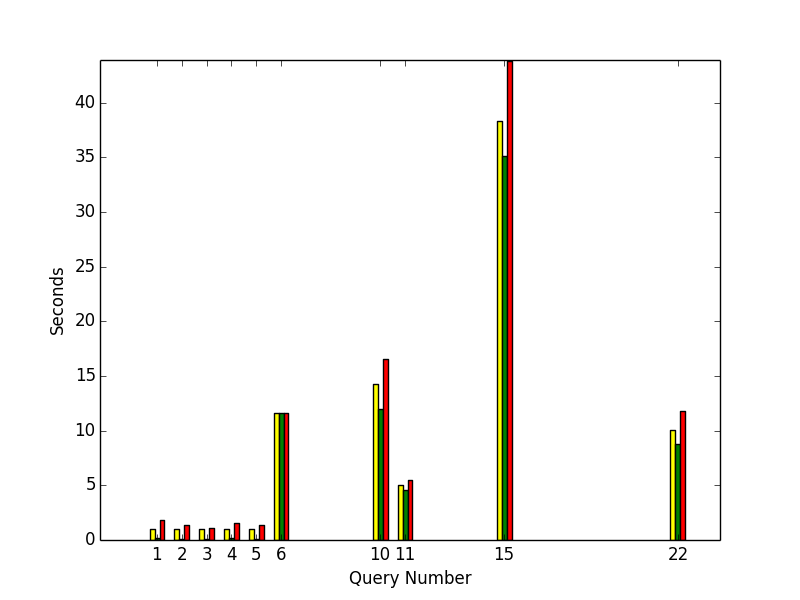
\includegraphics[width=\textwidth]{img/00_conf_initial}
\caption{Tempos de execução para cada \textit{query} \label{overflow}}
\end{figure}

Para uma identificação mais fácil das \textit{queries} do \textit{CHBenchmark} que foram executadas no gráfico acima, segue-se o que cada uma faz:
\\

\textbf{\textit{Query 1}} - Esta consulta informa a quantidade total e quantidade de todas as \textit{OrderLines} enviados dadas por um período de tempo específico. Além disso, informa sobre a quantidade média e quantidade mais a contagem total de todos esses \textit{OrderLines} ordenados pelo número \textit{OrderLine} individual.

\begin{verbatim}
select
  ol_number, sum(ol_quantity) as sum_qty, sum(ol_amount) as sum_amount, avg(ol_quantity) as avg_qty,
  avg(ol_amount) as avg_amount, count(*) as count_order
from
  order_line
where
  ol_delivery_d > '2007-01-02 00:00:00.000000'
group by
  ol_number
order by
  ol_number
\end{verbatim}


\textbf{\textit{Query 5}} – Esta consulta serve para obter informações sobre as receitas conseguidas das nações dentro de uma determinada região. Todas as nações são classificadas segundo o valor total da receita adquirida desde a data indicada.

\begin{verbatim}
select n_name,sum(ol_amount) as revenue
from customer, oorder, order_line, stock, supplier, nation, region
where c_id = o_c_id
     and c_w_id = o_w_id
     and c_d_id = o_d_id
     and ol_o_id = o_id
     and ol_w_id = o_w_id
     and ol_d_id=o_d_id
     and ol_w_id = s_w_id
     and ol_i_id = s_i_id
     and mod((s_w_id * s_i_id),10000) = su_suppkey
     and ascii(substr(c_state,1,1)) = su_nationkey
     and su_nationkey = n_nationkey
     and n_regionkey = r_regionkey
     and r_name = 'Europe'
     and o_entry_d >= '2007-01-02 00:00:00.000000'
group by n_name
order by revenue desc;
\end{verbatim}


\textbf{\textit{Query 6}} – Esta consulta lista o montante total das receitas arquivadas do OrderLines que foram entregues num período específico e uma certa quantidade.

\begin{verbatim}
select
  sum(ol_amount) as revenue
from
  order_line
where
  ol_delivery_d >= '1999-01-01 00:00:00.000000'
  and ol_delivery_d < '2020-01-01 00:00:00.000000'
  and ol_quantity between 1 and 100000
\end{verbatim}

\textbf{\textit{Query 10}} – Esta consulta serve para analisar as despesas de todos os clientes listagem o seu país, alguns detalhes deles e a quantidade de dinheiro que eles têm usado para tomar as suas ordens desde uma data específica. A lista inteira é ordenada pela quantidade de encomendas dos clientes.

\begin{verbatim}
select
  c_id, c_last, sum(ol_amount) as revenue, c_city, c_phone, n_name
from
  customer, oorder, order_line, nation
where
  c_id = o_c_id
  and c_w_id = o_w_id
  and c_d_id = o_d_id
  and ol_w_id = o_w_id
  and ol_d_id = o_d_id
  and ol_o_id = o_id
  and o_entry_d >= '2007-01-02 00:00:00.000000'
  and o_entry_d <= ol_delivery_d
  and n_nationkey = ascii(substr(c_state,1,1))
group by
  c_id, c_last, c_city, c_phone, n_name
order by
  revenue desc
\end{verbatim}


\textbf{\textit{Query 17}} – Esta consulta determina a perda anual de receita, se as encomendas apenas com uma quantidade de mais do que a quantidade média de todas as ordens no sistema fosse tomadas e enviadas aos clientes.

\begin{verbatim}
select
  sum(ol_amount) / 2.0 as avg_yearly
from
  order_line, (
  select
    i_id, avg(ol_quantity) as a
  from
    item, order_line
  where
    i_data like '%b' and ol_i_id = i_id group by i_id) t
where
  ol_i_id = t.i_id and ol_quantity < t.a
\end{verbatim}


Posto isto chegou-se à conclusão que é necessário avaliar as 5 \textit{queries} do \textit{CHBenchmark} que foram executadas e que tiveram um tempo de execução muito elevado, ou seja, verificar o que se passa nas mesmas e tentar melhor o seu desempenho. Um dos pontos que foi possível concluir é que estas \textit{queries} apresentadas têm um tempo de execução elevado porque possuem várias condições para as mesmas serem realizadas com sucesso. Após análise às mesmas foi possível concluir que em apenas duas conseguimos melhorar o desempenho alterando o código \textit{SQL} da mesma sem afetar a base de dados.\\

\newpage

\subsection{Desempenho \textit{Query 1}}

Na \textit{query 1} com o código seguinte, conseguimos melhorar a performance levando menos tempo a executar a query e obtendo o mesmo resultado, simplesmente dividindo a \textit{query} em dois \textit{select} de forma a melhorar a performance como é demonstrado a seguir:

\begin{verbatim}
select ol_number,
  sum_qty,
  sum_amount,
  sum_qty/count_order as avg_qty,
  sum amount/count_order as avg_amount,
  count_order
from
  (select
    ol_number, sum(ol_quantity)as sum_qty, sum(ol_amount) as sum_amount, count(*) as count_order
  from
    order_line
  where
    ol_delivery_d > '2007-01-02 00:00:00.000000'
    group by ol_number
    order by ol_number) as t
\end{verbatim}

\begin{figure}[ht!]
\centering
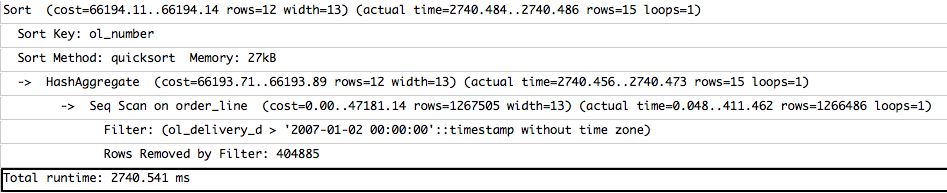
\includegraphics[width=\textwidth]{img/00_query1_pos}
\caption{Plano de execução da \textit{query 1} antes da otimização \label{overflow}}
\end{figure}

\begin{figure}[ht!]
\centering
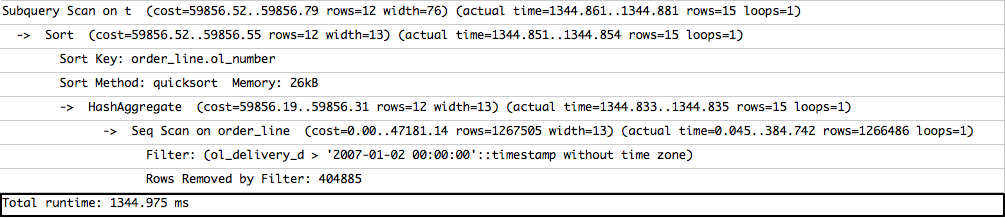
\includegraphics[width=\textwidth]{img/00_query1_ant}
\caption{Plano de execução da \textit{query 1} depois da otimização \label{overflow}}
\end{figure}

Como é possivel visualizar nas figuras acima obtivemos uma melhoria de desempenho, onde conseguimos reduzir para menos de metade o tempo total de execução da \textit{query}. Como podemos confirmar a otimização foi efetuada corretamente isto porque os resultados obtidos são exatamente os mesmos. Como é possivel verificar, dividindo a \textit{query} em duas \textit{queries} ou efetuado uma \textit{sub-query} conseguimos reduzir para metade o tempo de execução, isto porque primeiro os dados são selecionados de acordo com as condições pedidas e só depois na \textit{query} principal é que são mostrados os dados que interessam.

\newpage

\subsection{Desempenho \textit{Query 17}}

Na \textit{query 17} foi possível fazer algumas melhorias, isto porque a mesma fica mais eficiente se houver uma \textit{materialized view} para calcular a média para cada índice. Segue-se abaixo o código \textit{SQL} que permite obter os mesmos resultados mas com mais eficiência e os respetivos planos de execução para comparação:

\begin{verbatim}
CREATE MATERIALIZED VIEW AvgByID AS
  select i_id, avg(ol_quantity) as average
  from item, order_line
  where i_data like '%b' and ol_i_id = i_id
  group by i_id

select
  sum(ol_amount) / 2.0 as avg_yearly
from
  order_line,
  (select
    i_id, average
  from
    AvgByID) t
where
  ol_i_id = t.i_id
  and ol_quantity < t.average
\end{verbatim}

\begin{figure}[ht!]
\centering
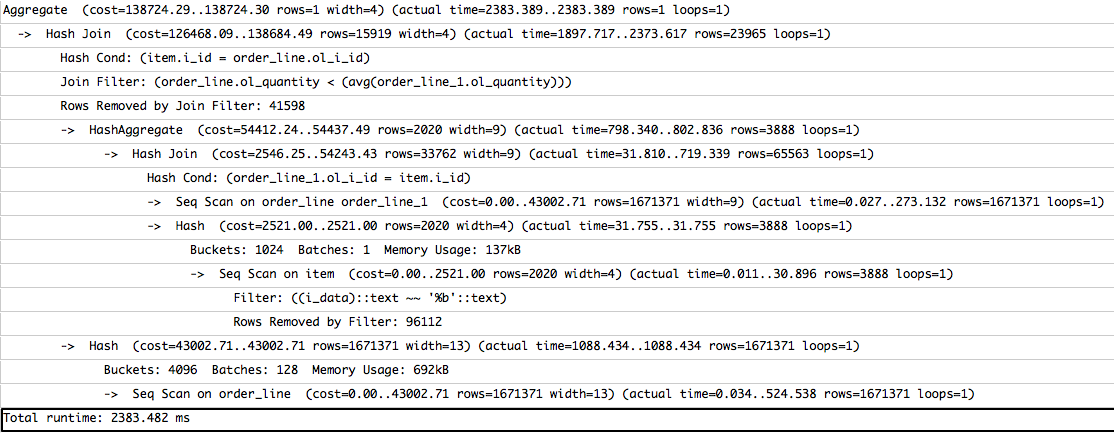
\includegraphics[width=\textwidth]{img/00_query17_ant}
\caption{Plano de execução da \textit{query 17} antes da otimização \label{overflow}}
\end{figure}

\begin{figure}[h!]
\centering
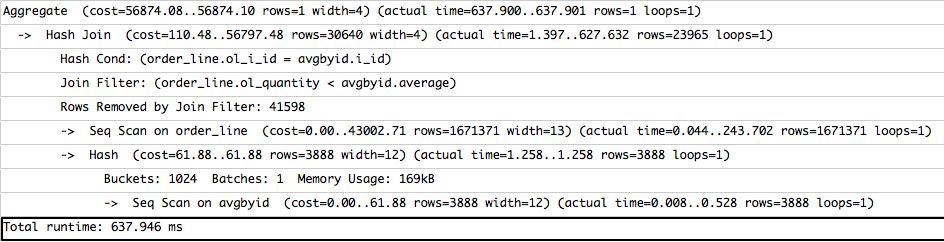
\includegraphics[width=\textwidth]{img/00_query17_pos}
\caption{Plano de execução da \textit{query 17} depois da otimização \label{overflow}}
\end{figure}


No melhoramento desta \textit{query} é possivel visualizar que através duma \textit{materialized view}, conseguimos reduzir drasticamente o tempo de execução da \textit{query}. Neste caso, como o pretendido é consultar os dados e não altera-lós a \textit{materialized view} encaixa como um possivel método de visualização, isto porque apesar de ocupar mais espaço na nossa base de dados, ficamos com os dados que pretendemos ver pré-compilados tendo assim uma melhoria elevada de perfomance aquando duma consulta da \textit{materialized view}. A \textit{materialized view} permite que os cálculos sejam feitos previamente e assim ao contrário das \textit{views} normais que consultam os dados em tempo de execução perdendo assim desempenho. 

\newpage

\subsection{Desempenho das restantes \textit{queries}}

Analisando a \textit{query 5} pode-se ver que o tempo de execução da mesma é elevado porque a condição \textit{where} é bastante extensa, tendo várias condições que são feitas uma a uma, diminuindo assim o desempenho da mesma.\\

Analisando a \textit{query 6} é possível notar que a mesma tem uma longa duração de execução devido às condições impostas na condição \textit{where}. A gama de valores é bastante elevada tendo de percorrer cerca de 20 anos de registos bem como a quantidade presente que pode variar entre valores muito elevados (1 a 100000).\\

Analisando a \textit{query 10} é possível notar que o que esta a fazê-la perder performance é o facto de estar a fazer um \textit{group by} muito grande, o que leva a que o custo da query seja maior e a mesma demore mais tempo a ser executada.\\

\textit{Os planos de execução destas queries encontram-se em anexo.}
